\documentclass[xcolor={dvipsnames}]{beamer}

% Paquets utilisés
\usepackage{animate} % pour faire des animations
\usepackage{listings} % pour insérer des lignes de codes avec de la coloration syntaxique
\usepackage[audience=english]{beameraudience}  % pour écrire la présentation en 2 langues
\usepackage{textpos} % pour positionner des figure où l'on veut
\usepackage{tikz} % pour faire de jolies figures
\usepackage{pifont} % pour avoir des symboles sympa

\usetikzlibrary{shapes.geometric} % pour faire des logigrammes avec TikZ
\usetikzlibrary{arrows.meta}
\tikzset{%
  >={Latex[width=1mm,length=1mm]},
  % Specifications for style of nodes:
     note/.style  = {rectangle, minimum width=1cm, minimum height=0.3cm, align=left},
     bstep/.style = {rectangle, rounded corners, draw=black,
                     minimum width=1cm, minimum height=0.3cm, text centered},
     gstep/.style = {rectangle, rounded corners, draw=Green, fill=Green!10,
                     minimum width=1cm, minimum height=0.3cm, text centered},
     rstep/.style = {rectangle, rounded corners, draw=red, fill=red!10,
                     minimum width=1cm, minimum height=0.3cm, text centered},
     gtest/.style = {diamond, aspect=3., rounded corners, draw=Green, fill=Green!10,
                     minimum width=1cm, minimum height=0.3cm, text centered},
     rtest/.style = {diamond, aspect=3., rounded corners, draw=red, fill=red!10,
                     minimum width=1cm, minimum height=0.1cm, text centered},
}




% Thème et options générales de mise en forme
\usetheme{Singapore}
\usecolortheme{rose}
\setbeamertemplate{page number in head/foot}[totalframenumber] % pour ajouter les numéros des pages
\setbeamertemplate{navigation symbols}{} % pour virer les symboles "page suivantes" ...
\makeatletter % pour avoir des puces de progression
\setbeamersize{
  text margin left = 0.2cm, % modification des marges (normalement c'est 1 cm)
  text margin right = 0.2cm}
\setbeamertemplate{block begin}{  % pour ajuster la taille des block
  \begin{minipage}{.87\textwidth}%
    \begin{beamerboxesrounded}[upper=block title,lower=block body,shadow=true]{
    \raggedright\usebeamerfont*{block title}\insertblocktitle}
    \raggedright
    \usebeamerfont{block body}}
  \setbeamertemplate{block end}
{\end{beamerboxesrounded}\end{minipage}\vskip\smallskipamount}
\setlength{\unitlength}{1cm}

% Ajout de la description du language Gibiane (pour le paquet "listings")
\lstdefinelanguage{gibiane}{
  morekeywords=[1]{
      opti, born, dens, droi, lapl, cerc, mota, oper,
      quel, inte, para, et  , poin, plus, moin, tran, lister,
      rota, trac, inve, cote, elem, cont, diff, chan, list,
      surf, conf, info, tour, homo, affi, syme, incl, elim,
      titr, racc, tass, sort, lire, bary, dall, orie, manu,
      oubl, comp, cout, pave, comm, noeu, nbel, nbno,
      noti, face, coor, norm, temp, volu, lect, sauf, prog,
      +   , -   , *   , /   , **  , flot, enti, log , exp ,
      depl, psca, pvec, pmix, liai, regl, hook, sols, reso,
      date, rigi, bloq, depi, hota, stru, text, proj, venv,
      elst, jonc, reco, mass, clst, sigm, rela, forc, mome,
      vloc, base, dime, extr, vers, vibr, maxi, xtmx, ytmx,
      >   , <   , >eg , <eg , ou  , ega , non , neg , mult,
      pjba, crit, diag, xtx , uniq, bsig, deda, max1, mots,
      ipol, abs , sin , cos ,
      atg , enve, isov, detr, enle, remp, inse, coli, tria,
      tabl, redu, symt, anti, resu, pres, exco, nomc, saut,
      defo, appu, inva, prin, vmis, ksig, sign, suit, 
      valp, ordo, tire, rege, dess, amor, char, coul, chpo,
      afco, evol, orth, thet, comb, deve, vect, pica, capi, 
      copi, dimn, sauv, rest, cara, mate, gene,
      capa, elfe, jaco, plas, gree, mode, finp, xty ,
      debp, ktan, form, mess, nnor, cubp, cubt, cer3, fdt ,
      seis, ener, epsi, intg, cour, reac, supe, zero, depb,
      exci, kp  , acti, elas, erre, cong, lump, obte,
      vari, modi, masq, exis, mini, grad, ense, ifre, dfou,
      sigs, mapp, somm, brui, rten, dspr, tfr , tote,
      graf, tres, type, osci, spo , inde, chsp,
      tagr, perm, cabl, fofi, work, qulx, debi, 
      cmoy, comt, cond, flux, rimp, filt, tfri,
      conc, iter, acqu, sour, conv, acoh, psmo, asih, ecou,
      mena, synt, argu, atah, dyne, fonc, resp, plac,
      vale, proi, exce, aret, calp, indi, act3, biot,
      dedu, conn, nloc, chai, cosi, cvol, diad, hann, insi,
      lsqf, ltl , pert, prns, psrs, siar, spon, visa, cneq,
      ccon, mesu, pile, util, menu, cosh, sinh, tanh,
      deg3, aide, racp, refe, ksof, nske, kmab,
      noel, doma, fpu , gmv , eqpr, eqex, vibc, avct,
      kdia, kmtp, kmf , mdia, dfdt, tcrr, tcnm, sqtp, somt,
      nlin, cmct, kcht, lapn, raft, klop, kres, cson, %fimp, 
      nuag, weip, khis, kops, fsur, flam, elno,
      dbit, ns  , toim, kmbt, kbbt, dudw, frot, tsca,
      konv, kcha, mhyb, matp, hdeb, hvit, hybp, smtp, divu,
      mocu, chau, tail, erf , sens, impo, dans, impf, ntab,
      fron, fuit, epth, fpt , kfpt, fpa , kfpa, echi, qond,
      kpro, ffor, raye, rayn, vsur, traj, aju1, aju2, frig,
      excf, nomm, prec, erfc, onde, cfl , dedo, dcov, parc,
      pola, chi1, chi2, pent, pret, meth, xxt , cblo, genj,
      zleg, mesm, fion, neut, logk, coac, resi, mutu, sore,
      diri, lign, obje, debm, finm, heri, deco, exte, dmmu,
      dmtd, bmtd, ssch, mrem, assi, fiss, prim, annu, prob,
      sais, choi, deto, part, clmi, pmat, excp, prop, phaj,
      alea, gnfl, mpro, sste, adve, bgmo, ecfe, coup, verm,
      dfer, gyro, cori, kent, fant, itrc, reto, ijet, impe,
      moca, levm, ravc, idli, raff, cfnd, adet, psip, acos,
      asin, tan , trie, gane, hist, etg , oter, xfem, rfco,
      vide, voro, prra, posi, mise, misl, coll, pod,  
      option, borne, droit, droite, point, moins, titre,
  },
  morekeywords=[2]{  % quelques procedures
    pasapas, peche, explorer, @vecoul, vecflu
  },
  morekeywords=[3]{  % operateurs speciaux
    si, sino, sinon, fins, finsi, repe, repeter, quit, fin
  },
  sensitive=false, % mots clefs non sensibles à la casse
  morecomment=[f]*, % indique que les commentaires ont des * en 'first' colonne
  morestring=[b]', % indique que les chaines sont définies entre simples quotes
  moredelim=[is][\sffamily\slshape\color{blue}]{/*}{*/}
}
\definecolor{bckg}{rgb}{0.96,0.96,0.96}
\lstset{
%  language={gibiane},
%  backgroundcolor=\color{white},
  upquote=true,
  keywordstyle=[1]\color{red}\bfseries,
  keywordstyle=[2]\color{orange}\bfseries,
  keywordstyle=[3]\color{blue}\bfseries,
  commentstyle=\color{Aquamarine},
  stringstyle=\color{Green},
  basicstyle=\ttfamily\scriptsize,
  %captionpos=b, % Position of the Caption (t for top, b for bottom)
  %extendedchars=true, % Allows 256 instead of 128 ASCII characters
  tabsize=2, % number of spaces indented when discovering a tab 
  columns=fixed, % make all characters equal width
  keepspaces=true, % does not ignore spaces to fit width, convert tabs to spaces
  showstringspaces=false, % lets spaces in strings appear as real spaces
  breaklines=true, % wrap lines if they don't fit
  %frame=tb, % draw a frame at the top, right, left and bottom of the listing
  %frameround=tttt, % make the frame round at all four corners
  %framesep=4pt, % quarter circle size of the round corners
  %framexleftmargin=2mm, framexrightmargin=2mm,
  %framextopmargin=2mm,framexbottommargin=2mm,
  %frame=shadowbox, rulesepcolor=\color{gray},
  xrightmargin=5mm,
  belowskip=0pt
}


% Infos générales : titre / sous titre / date / auteur / organisme ...
\justfor{french}{
  \title{Cast3M~: la procédure PASAPAS}
  \subtitle{et les procédures utilisateurs}
  \date{Automne 2024}}
\justfor{english}{
  \title{Cast3M: the PASAPAS procedure}
  \subtitle{and the user's procedures}
  \date{Fall 2024}}
\author{François Di Paola}
\institute{CEA Saclay,\\
\url{http://www-cast3m.cea.fr}}

% Quelques raccourcis perso
\newcommand{\fe}[2]{\justfor{french}{#1}\justfor{english}{#2}}
\newcommand{\g}[1]{\textbf{#1}}
\newcommand{\tou}[1]{\underline{#1}}
\newcommand{\tod}[1]{\underline{\underline{#1}}}
\newcommand{\kw}[1]{\mbox{\texttt{#1}}}
\newcommand{\kwr}[1]{\textcolor{red}{\kw{#1}}}
\newcommand{\kwo}[1]{\textcolor{orange}{\kw{#1}}}
\newcommand{\kwg}[1]{\textcolor{Green}{\kw{#1}}}
\newcommand{\kwb}[1]{\textcolor{blue}{\kw{#1}}}
\newcommand{\kwv}[1]{\textcolor{Purple}{\kw{#1}}}
\newcommand{\red}[1]{\textcolor{red}{#1}}
\newcommand{\orange}[1]{\textcolor{orange}{#1}}
\newcommand{\green}[1]{\textcolor{Green}{#1}}
\newcommand{\blue}[1]{\textcolor{blue}{#1}}
\newcommand{\violet}[1]{\textcolor{Purple}{#1}}
\newcommand{\gray}[1]{\textcolor{gray}{#1}}
\newcommand{\white}[1]{\textcolor{white}{#1}}
\newcommand{\grille}{\draw[help lines,xstep=.1,ystep=.1] (0,0) grid (1,1);
                     \foreach \x in {0,1,...,9} { \node [anchor=north] at (\x/10,0) {0.\x}; }
                     \foreach \y in {0,1,...,9} { \node [anchor=east] at (0,\y/10) {0.\y}; }}
\newcommand{\avous}[1]{\orange{\ding{43}\emph{#1}}}
\newcommand{\tx}[1]{\textsf{#1}}


\begin{document}


\begin{frame}
  \titlepage
\end{frame}

%\begin{frame}{\fe{Sommaire}{Summary}}
%  \begin{itemize}
%    \item \fe{\hyperlink{rappels}{Rappels sur Cast3M et PASAPAS}}
%             {\hyperlink{rappels}{Reminders reminders on Cast3M and PASAPAS}}
%    \item \fe{\hyperlink{pasapas}{Fonctionnement de PASAPAS}}
%             {\hyperlink{pasapas}{How works PASAPAS}}
%    \item \fe{\hyperlink{unpas}{\blue{Équilibre mécanique statique} - procédure UNPAS}\\
%              $\rightarrow$ exercice 1~: \blue{force suiveuse}\\
%              $\rightarrow$ exercice 2~: \blue{rupture par suppression d'éléments}}
%             {\hyperlink{unpas}{\blue{Mechanical static equilibrium} - procedure UNPAS}\\
%              $\rightarrow$ exercice 1: \blue{following force}\\
%              $\rightarrow$ exercice 2: \blue{fracture by elements removal}}
%    \item \fe{\hyperlink{transnon}{\red{Équilibre thermique} - procédure TRANSNON}\\
%              $\rightarrow$ exercice 3~: \red{source de chaleur variable}\\
%              $\rightarrow$ exercice 4~: \red{contact thermo} \blue{mécanique}}
%             {\hyperlink{transnon}{\red{Thermal equilibrium} - procedure TRANSNON}\\
%              $\rightarrow$ exercice 3: \red{variable heat source}\\
%              $\rightarrow$ exercice 4: \red{thermo} \blue{mechanical} \red{contact}}
%  \end{itemize}
%\end{frame}

%% Remplacer les apostrophes ’ par des quotes '
% Exo 1 : mettre les grands deplacements initialement


\begin{frame}{\fe{Exercice 3 : dépendance à la température}
                 {Exercise 3: temperature-dependence}}
             {\fe{Solution avec PERSO2}{Solution with PERSO2}}
  \footnotesize
  \begin{itemize}
    \small
    \item \fe{Utiliser la procédure \kwv{PERSO2}}{Use procedure \kwv{PERSO2}}
  \end{itemize}
  \vspace{4.5cm}
  \scriptsize
  \begin{textblock*}{10cm}(0.3cm,-3.2cm)
    \fe{\emph{Programme principal}}{\emph{Main program}}
  \end{textblock*}
  \begin{textblock*}{10cm}(6.2cm,-4cm)
    \fe{\emph{\violet{Procédure PERSO2}}}{\emph{\violet{PERSO2 procedure}}}
  \end{textblock*}
\end{frame}

\begin{frame}{\fe{Exercice 3 : dépendance à la température}
                 {Exercise 3: temperature-dependence}}
  \footnotesize
  \begin{itemize}
    \item \fe{Résultats}{Results}\\
    \hspace{1cm}
  \end{itemize}
\end{frame}

%%%%%%%%%%%%%%%%%%%%%%%%%%%%%%%%%%%%%%%%%%%%
\fe{\section{Rappels}}{\section{Reminders}}
\label{rappels}
%%%%%%%%%%%%%%%%%%%%%%%%%%%%%%%%%%%%%%%%%%%

\begin{frame}{\fe{Cast3M, quid ?}{What is Cast3M?}}
  \begin{center}
    \fe{Logiciel de simulation utilisant la \g{méthode des éléments finis} en \g{mécanique/thermique} des \g{structures} et des \g{fluides}}
       {A simulation software using the \g{finite element method} in \g{thermal and mechanical} analysis of \g{structures} and \g{fluids}}\pause
  \end{center}
  \begin{itemize}
    \item \fe{Résolution d'\g{équations aux dérivées partielles}}
             {\g{Partial differential equations} solver}\pause
    \item \fe{\g{Système complet} : solveur, pré/post-processeur, visualisation, import/export des données\dots}
             {\g{Complete software}: solver, pre-processing and post-processing, visualization, reading/writing data\dots}\\~\\
    \begin{center}
      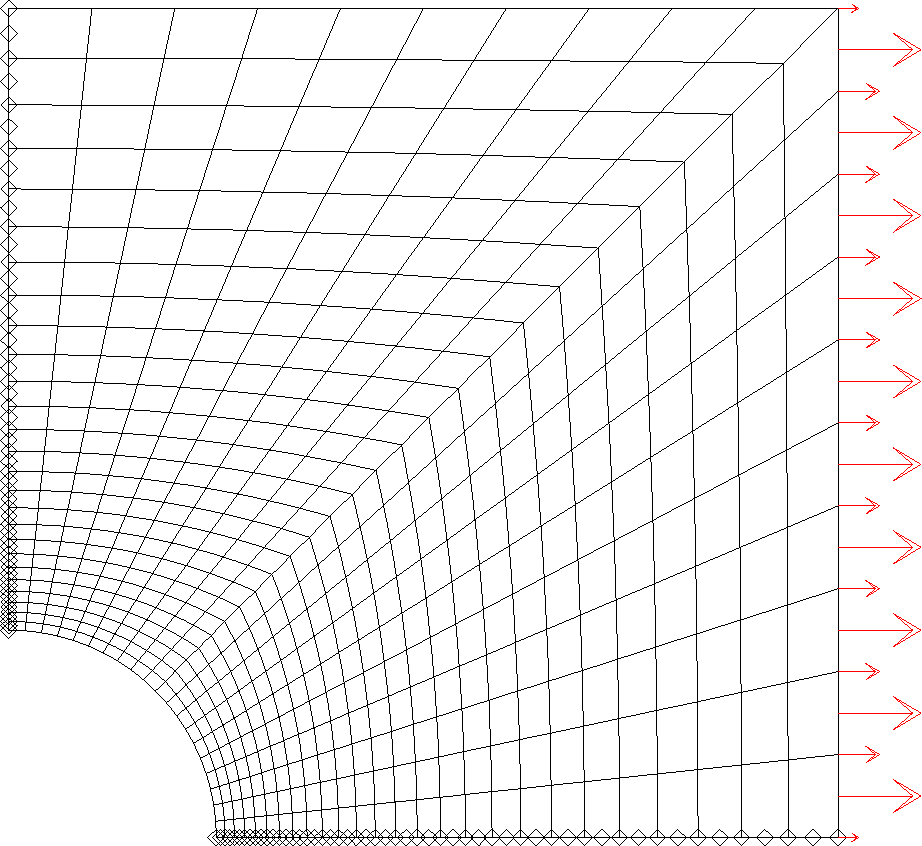
\includegraphics[height=0.25\textheight]{images/plaque.1} \:
      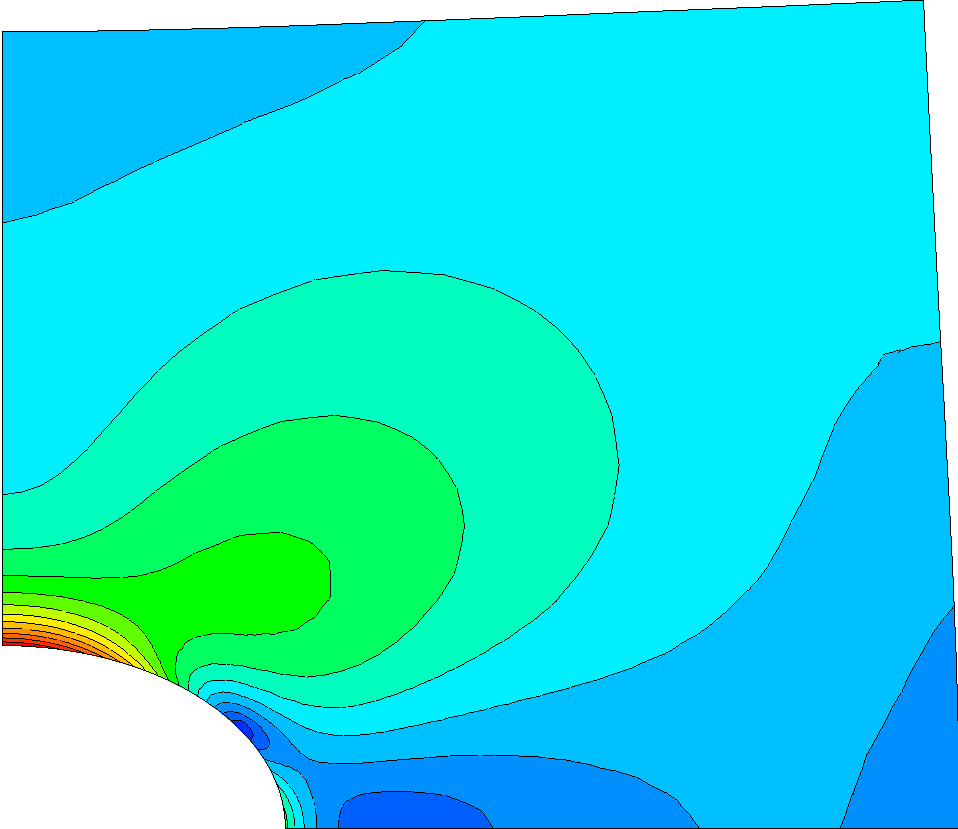
\includegraphics[height=0.25\textheight]{images/plaque.2} \:
      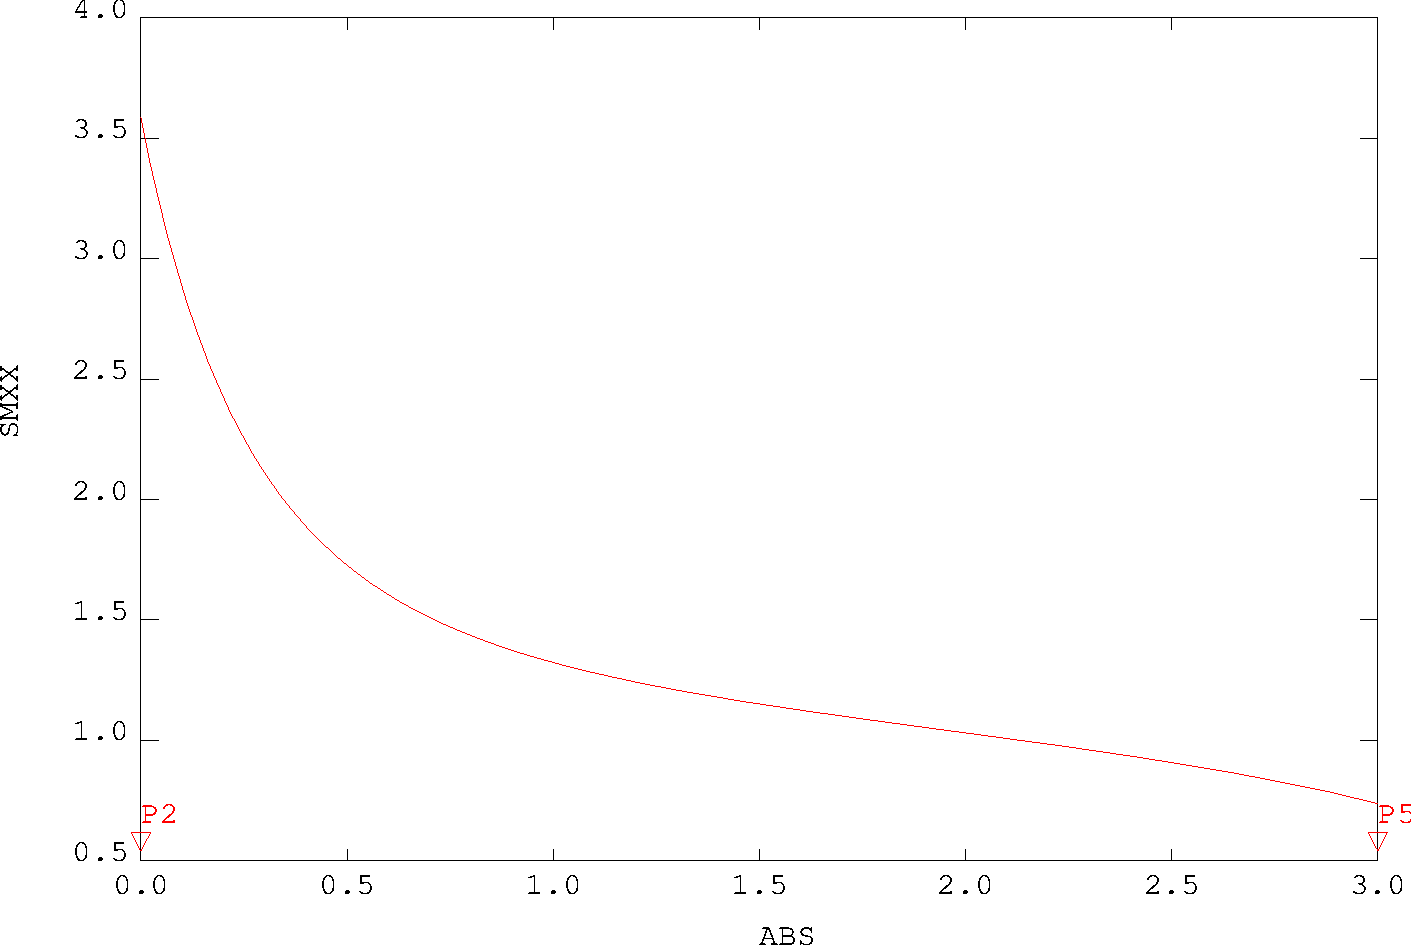
\includegraphics[height=0.25\textheight]{images/plaque.3}
    \end{center}\pause
    \item \fe{Basé sur un langage de commande : \g{Gibiane} (orienté objet)}
             {Based on a programming language: \g{Gibiane} (objet-oriented)}\\
  \end{itemize}
\end{frame}

\begin{frame}{\fe{Nombreux domaines d'application}{Wide range of applications}}
  \small{
  \begin{itemize}
    \item<1->\fe{\g{Mécanique des structures}}{\g{Structural mechanics}}\\
    \footnotesize{
    \fe{\red{Quasi-statique} (non linéarités matériau, géométrie, conditions limites)}
       {\red{Quasi-static} (non linear behavior, geometry, boundary conditions)}\\
    \onslide<1>{
      \begin{textblock*}{5cm}(2cm,0.3cm)
        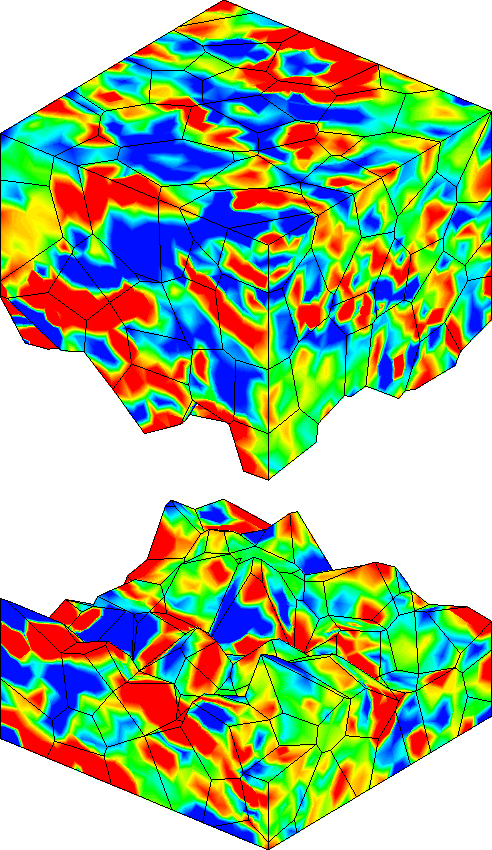
\includegraphics[height=0.4\textheight]{images/polycristal}
      \end{textblock*}
      \begin{textblock*}{5cm}(5cm,1.2cm)
        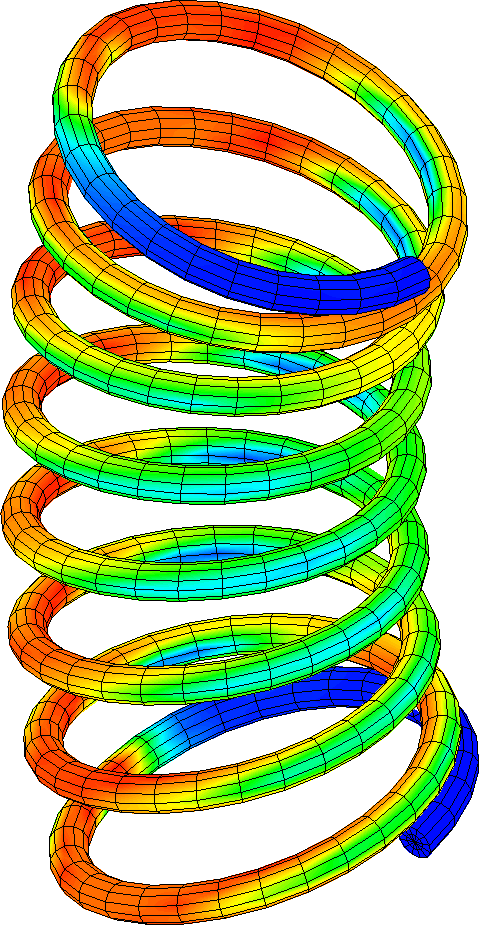
\includegraphics[height=0.4\textheight]{images/ressort}
      \end{textblock*}
      \begin{textblock*}{5cm}(8cm,2.1cm)
        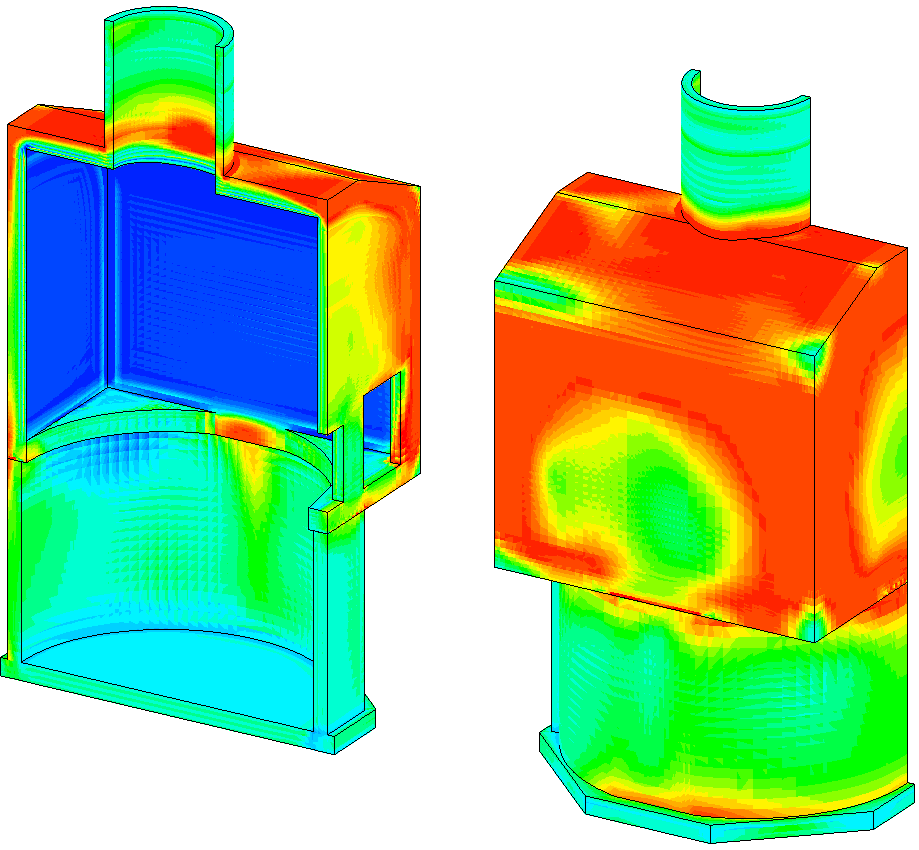
\includegraphics[height=0.4\textheight]{images/galatee}
      \end{textblock*}
      \begin{textblock*}{5cm}(9.4cm,5.6cm)
        \tiny{\emph{(S. Durand)}}
      \end{textblock*}}
    \onslide<2->\fe{\orange{Contact/frottement}, \green{Flambage}}
                    {\orange{Contact/friction}, \green{Buckling}}\\
    \onslide<2>{
      \begin{textblock*}{5cm}(1cm,0.3cm)
        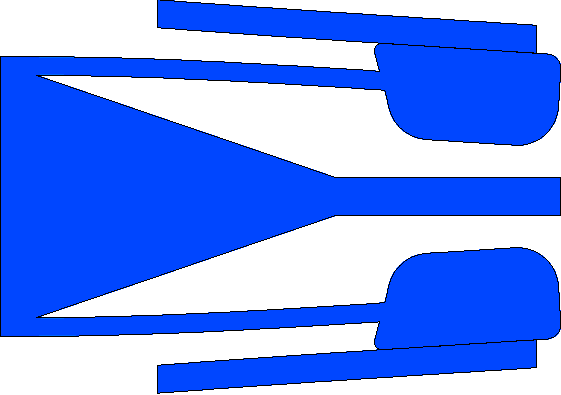
\includegraphics[height=0.25\textheight]{images/sac_a_dos.15}
      \end{textblock*}
      \begin{textblock*}{5cm}(4.8cm,0.3cm)
        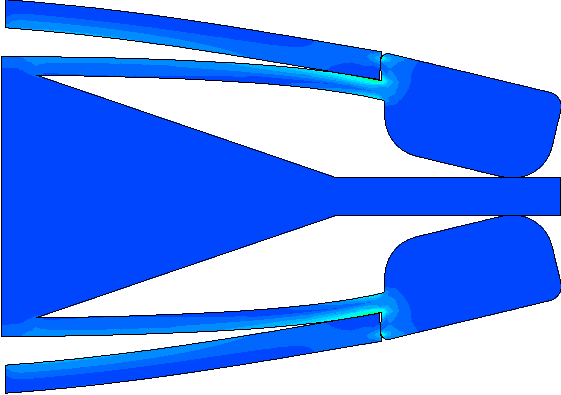
\includegraphics[height=0.25\textheight]{images/sac_a_dos.32}
      \end{textblock*}
    \begin{textblock*}{5cm}(8.5cm,0.3cm)
        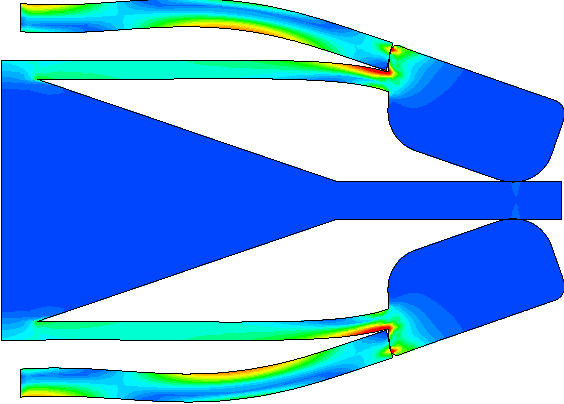
\includegraphics[height=0.25\textheight]{images/sac_a_dos.41}
      \end{textblock*}}
    \onslide<3->\fe{\blue{Dynamique} (temporelle, modale, interaction fluide structure)}
                    {\blue{Dynamic} (temporal, modal, fluid structure interaction)}\\
    \onslide<3>{
      \begin{textblock*}{5cm}(1cm,0.3cm)
        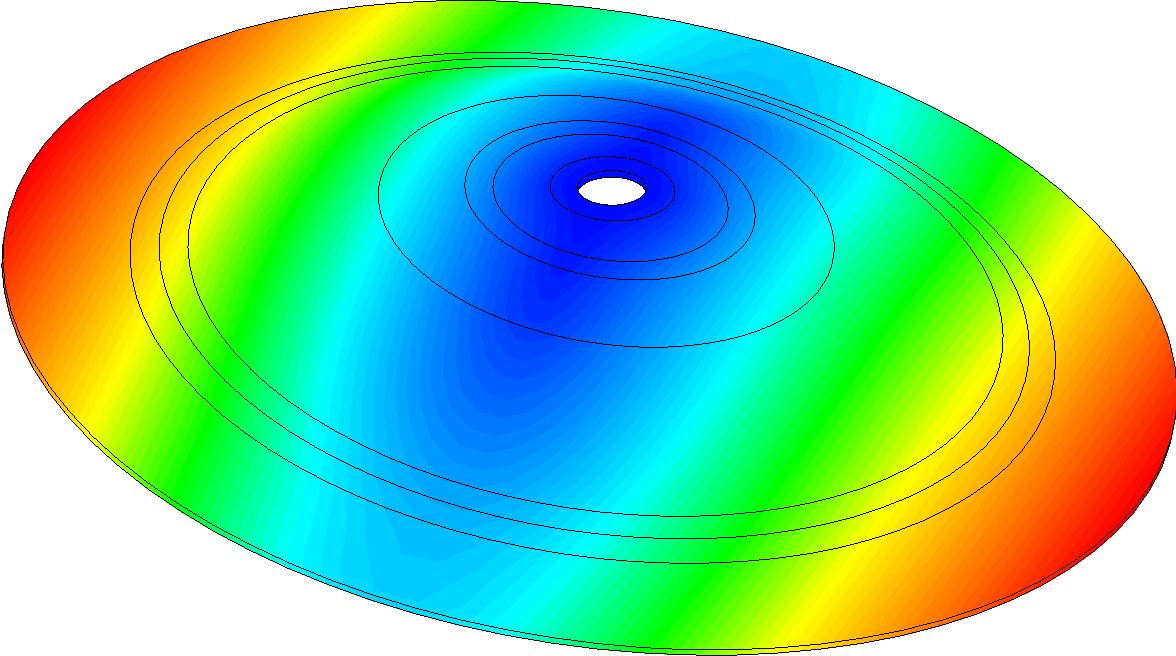
\includegraphics[height=0.2\textheight]{images/cymbale_mode_1}
      \end{textblock*}
      \begin{textblock*}{5cm}(4.8cm,0.3cm)
        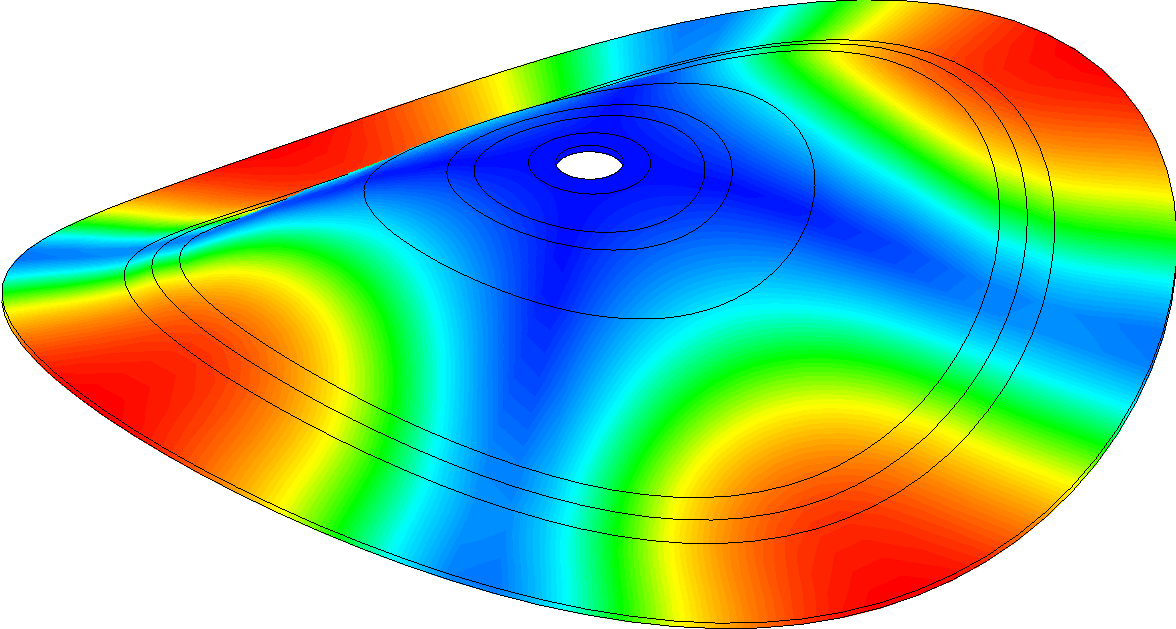
\includegraphics[height=0.2\textheight]{images/cymbale_mode_2}
      \end{textblock*}
      \begin{textblock*}{5cm}(8.5cm,0.3cm)
        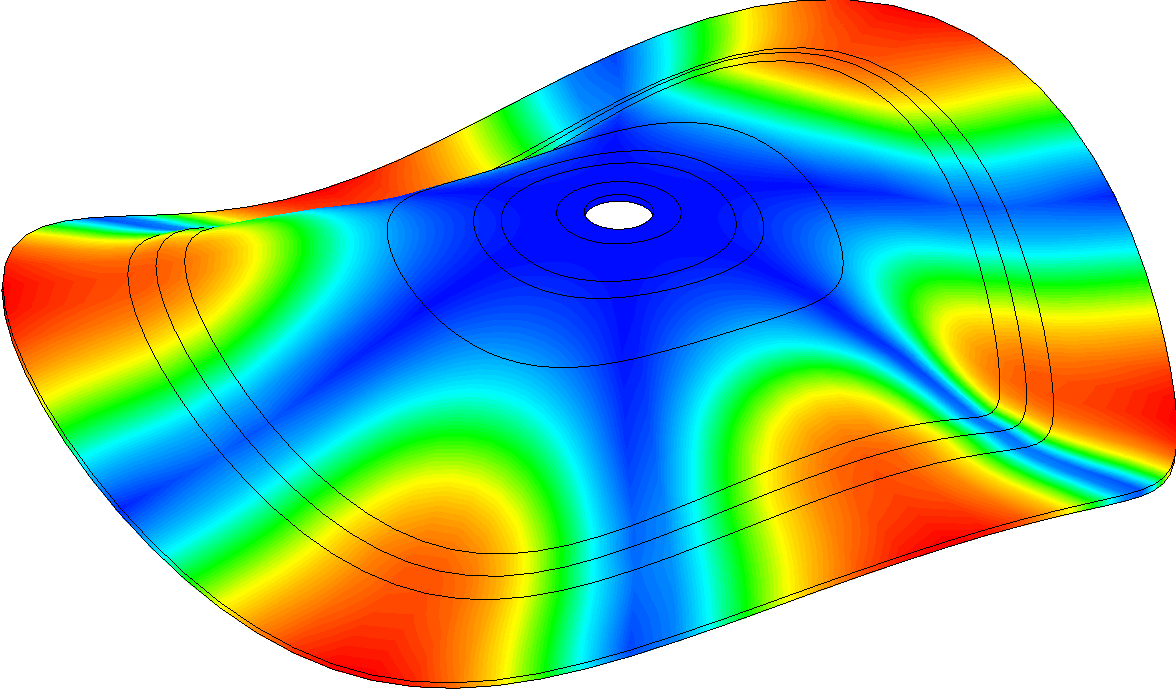
\includegraphics[height=0.2\textheight]{images/cymbale_mode_4}
      \end{textblock*}}
    \onslide<4->\fe{\violet{Rupture} (XFEM, propagation dynamique, zones cohésives)}
                   {\violet{Fracture} (XFEM, dynamic propagation, cohesive zones models)}\\
    \onslide<4>{
      \begin{textblock*}{12cm}(1.5cm,0.3cm)
        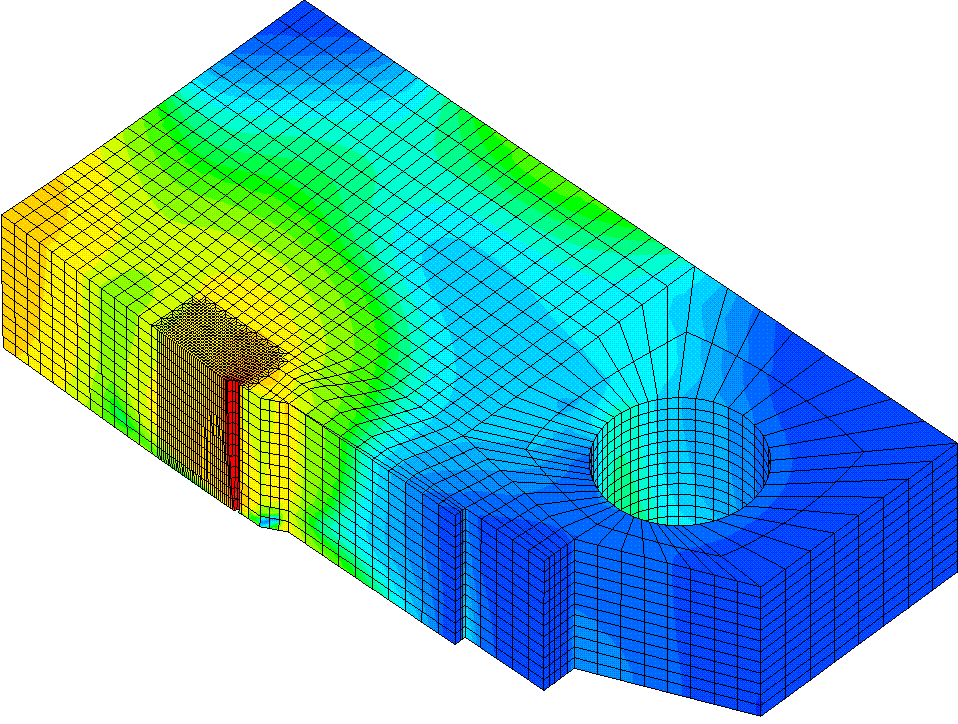
\includegraphics[height=0.25\textheight]{images/rousselier_03}
        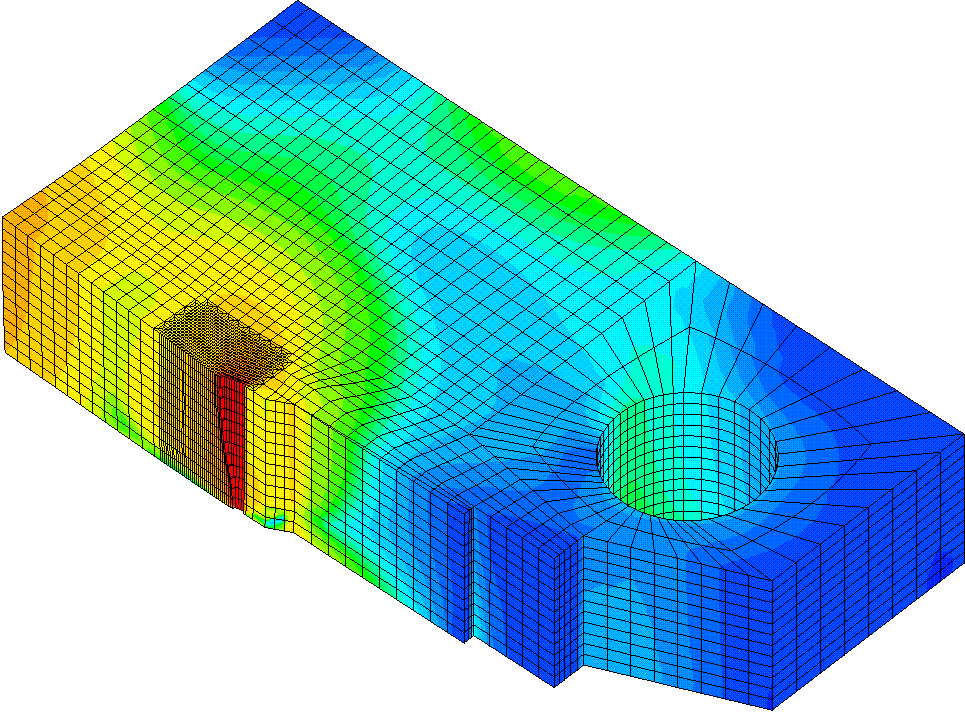
\includegraphics[height=0.25\textheight]{images/rousselier_04}
        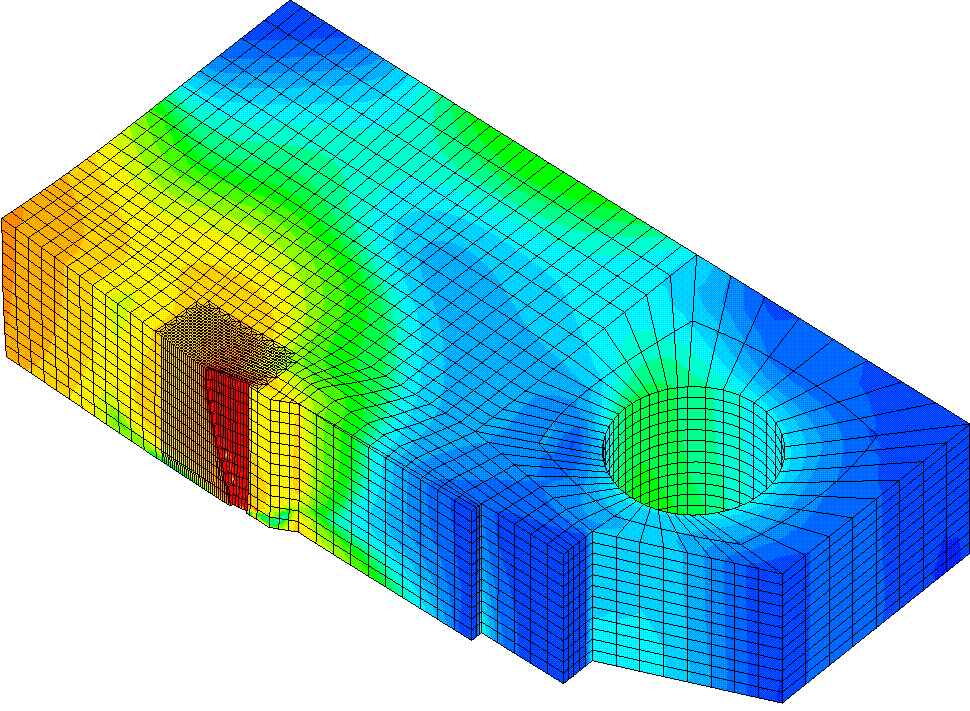
\includegraphics[height=0.25\textheight]{images/rousselier_05}\\
        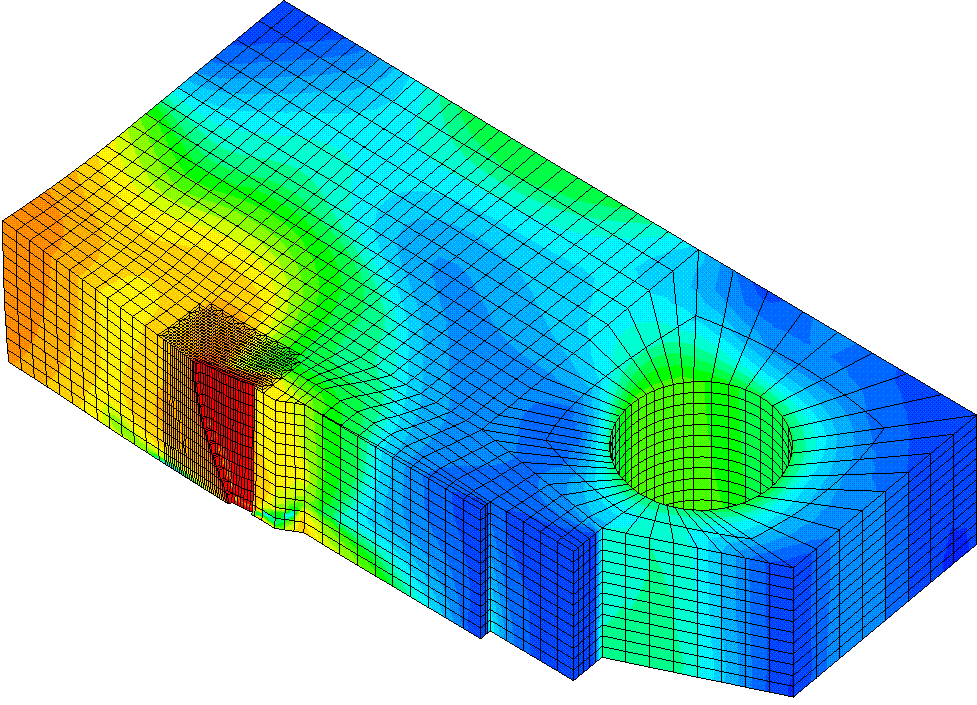
\includegraphics[height=0.25\textheight]{images/rousselier_06}
        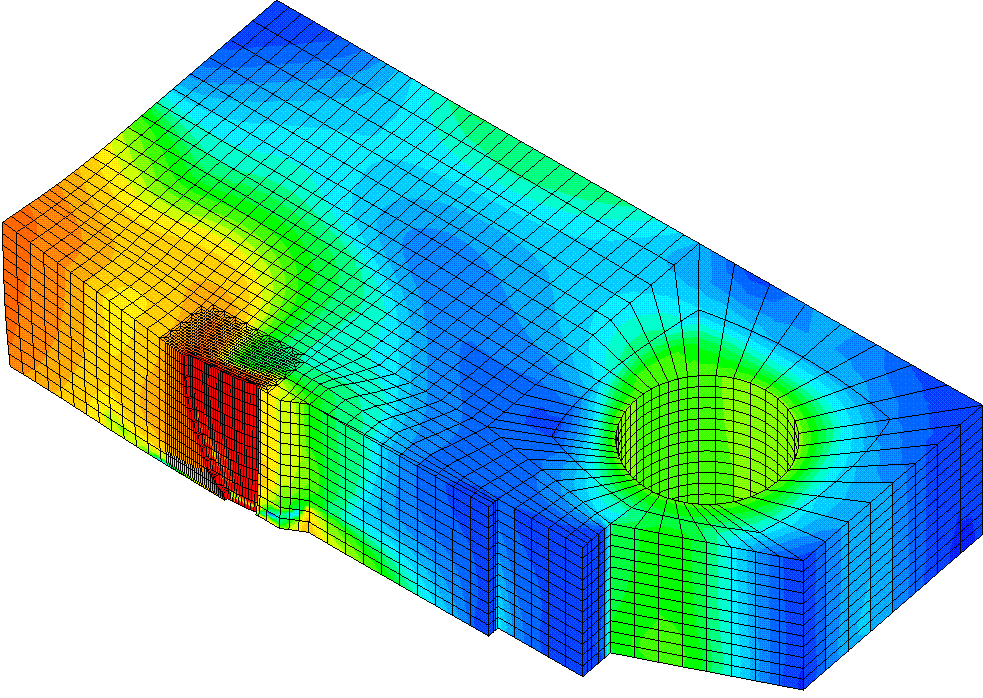
\includegraphics[height=0.25\textheight]{images/rousselier_07}
        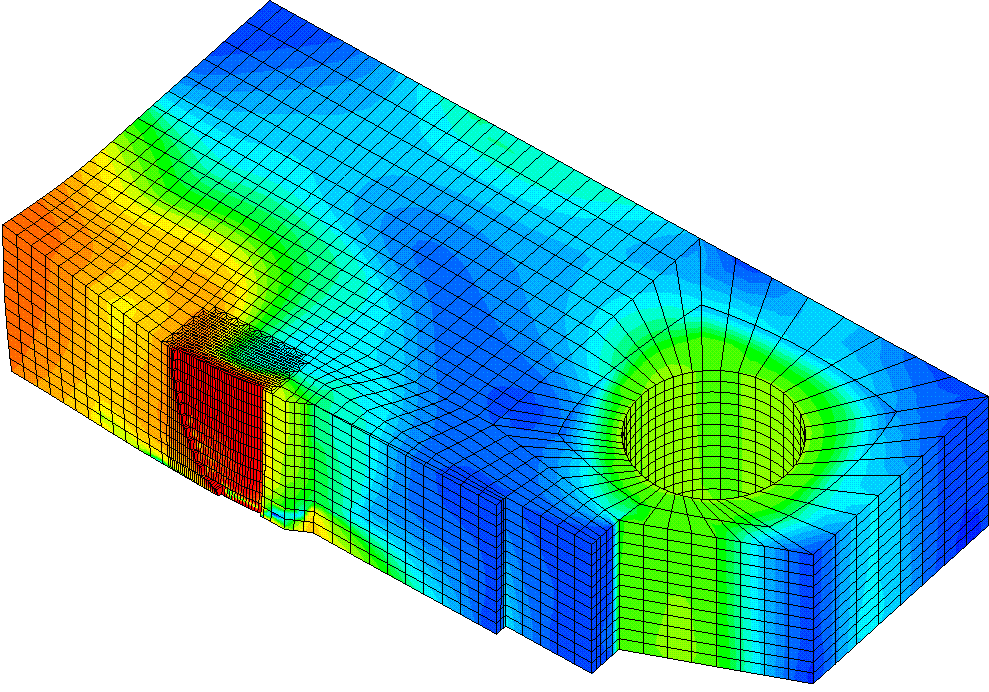
\includegraphics[height=0.25\textheight]{images/rousselier_08}
      \end{textblock*}
      \begin{textblock*}{5cm}(8cm,4.7cm)
        \tiny{\emph{(S. Kebiri)}}
      \end{textblock*}}
    \onslide<5>{
      \begin{textblock*}{12cm}(3.5cm,1.3cm)
        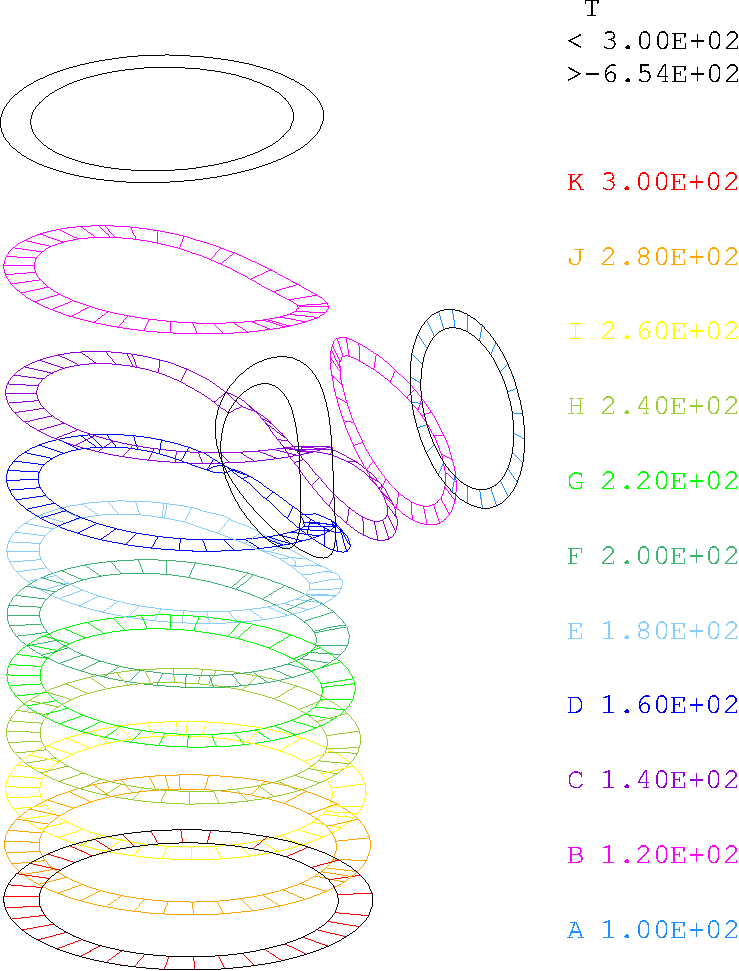
\includegraphics[height=0.4\textheight]{images/te_temperature}\hspace{1cm}
        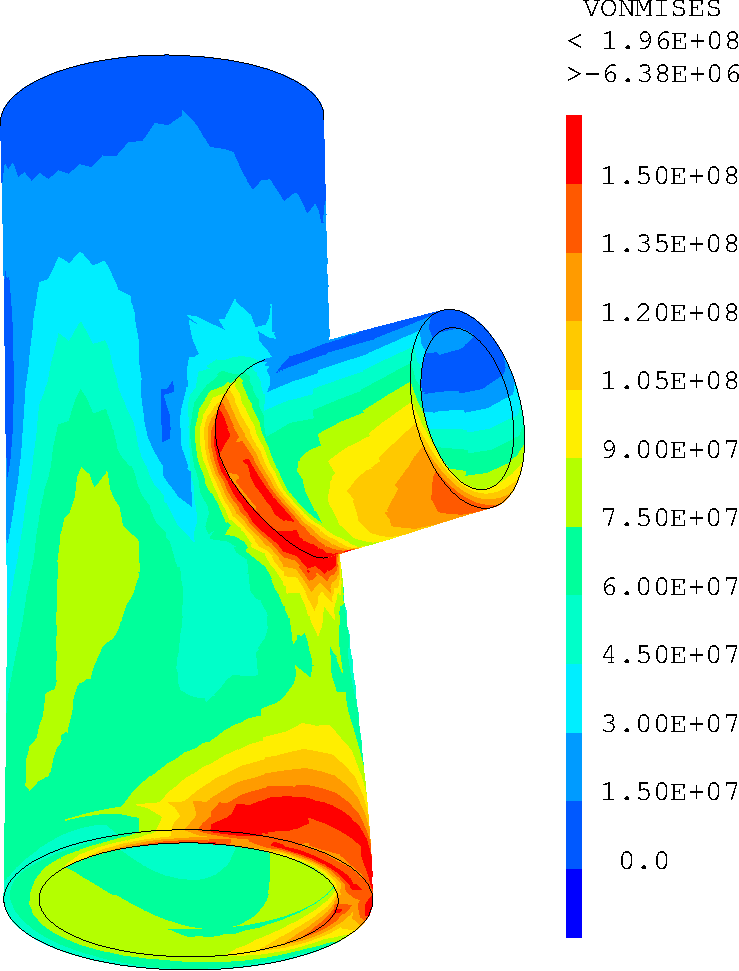
\includegraphics[height=0.4\textheight]{images/te_sigma}
      \end{textblock*}}
    \onslide<6>{
      \begin{textblock*}{12cm}(6.5cm,1.2cm)
        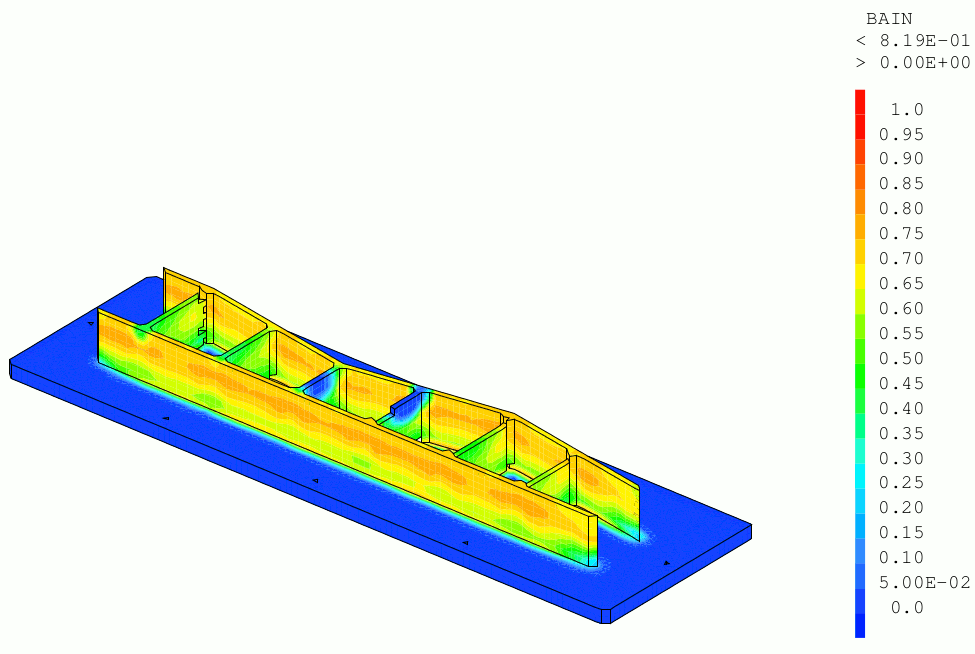
\includegraphics[height=0.4\textheight]{images/metallurgie}
      \end{textblock*}
      \begin{textblock*}{5cm}(8cm,4.7cm)
        \tiny{\emph{(C. Berthinier)}}
      \end{textblock*}}}
    \item<5->\fe{\g{Thermique}}{\g{Thermal analysis}}\\
    \footnotesize{
      \fe{Conduction, convection, rayonnement, changement de phase}
       {Conduction, convection, radiation, phase transition}}
    \item<6->\fe{\g{Mécanique des fluides}}{\g{Fluid mechanics}}
    \item<6->\fe{\g{Diffusion} multi espèces (loi de Fick)}{Multi species \g{diffusion} (Fick's law)}
    \item<6->\fe{Magnétostatique}{Magneto-statics}
    \item<6->\fe{Métallurgie}{Metallurgy}
    \item<6->\fe{Couplage thermo-hygro-mécanique}{Thermo-hygro-mechanics coupling}
  \end{itemize}}
\end{frame}

\begin{frame}{\fe{Présentation de PASAPAS}{The PASAPAS procedure}}
  \begin{itemize}
    \item \fe{Objectif}{Objective}\\
    \footnotesize
    \fe{Résolution de problèmes \emph{non linéaires évolutifs} de manière incrémentale\\
        en \red{thermique} et en \blue{mécanique}\\
        le temps peut être physique (ex~: thermique transitoire)\\
        ou non (ex~: plasticité avec chargement progressif)\\
        $\rightarrow$ on parle donc volontiers de \emph{variable d'évolution}\\}
       {Incremental solving of \emph{non linear progressive}\\
        \red{thermal} and \blue{mechanical} problems\\
        Time can be physical (e.g. thermal transients)\\
        or not (e.g. plasticity with progressive loading)\\
        $\rightarrow$ time or pseudo-time is called the \emph{evolution parameter}\\}
    ~
    \normalsize
    \item \fe{Types de non linéarités traitées}{Non linear phenomena considered}\\
    \fe{\red{Comportement} \footnotesize (plasticité, endommagement, matériaux variables, etc.) \normalsize\\
        \orange{Géométrie} \footnotesize (grands déplacements) \normalsize\\
        \green{Déformations} \footnotesize (grandes rotations) \normalsize\\
        \violet{Conditions limites} \footnotesize (rayonnement, frottement, pression suiveuse, etc.) \normalsize}
       {\red{Behavior} (plasticity, damage, variable material properties, etc.)\\
        \orange{Geometry} (large displacements)\\
        \green{Strains} (large rotations)\\
        \violet{Boundary conditions} (radiation, friction, following pressure, etc.)}
  \end{itemize}
\end{frame}

\begin{frame}{\fe{Utilisation de PASAPAS}{PASAPAS use}}
  \begin{itemize}
    \item \fe{\g{Créer une table} contenant toutes les données du problème}
             {\g{Create a table} containing all the data:}\\
    \lstinputlisting[language=gibiane, firstline=1, lastline=9]{dgibi/exemples.dgibi}
    \item \fe{\g{Appeler la procédure}}{\g{Procedure call:}}\\
    \lstinputlisting[language=gibiane, firstline=11, lastline=11]{dgibi/exemples.dgibi}
    \item \fe{\g{Post traitement} des résultats}{Results \g{post-processing}}
  \end{itemize}
\end{frame}

\begin{frame}{\fe{Aperçu des paramètres d'entrée}{Overview of input parameters}}
  \begin{itemize}
    \item \fe{Généralités}{General}\\
    \tiny
    \begin{tabular}{lll}
    \kwg{'MODELE'}           & MMODEL   & \fe{Équations à résoudre, formulation EF (\kwr{MODE})}
                                             {Equations to solve, FE formulation (\kwr{MODE})}\\
    \kwg{'CARACTERISTIQUES'} & MCHAML   & \fe{Paramètres matériau et/ou géométriques (\kwr{MATE})}
                                             {Material and/or geometrical parameters (\kwr{MATE})}\\
    \kwg{'CHARGEMENT'}       & CHARGEME & \fe{Évolution des CL et chargements au cours du calcul (\kwr{CHAR})}
                                             {BC and loading variation during calculation (\kwr{CHAR})}\\
    \end{tabular}
    \normalsize
    \item \fe{Thermique}{Thermal analysis}\\
    \tiny
    \begin{tabular}{lll}
    \kwg{'BLOCAGES\_THERMIQUES'} & RIGIDITE & \fe{Matrice de blocage des CL de type Dirichlet (\kwr{BLOQ})}
                                                 {Stiffness matrix for Dirichlet BC (\kwr{BLOQ})}\\
    \kwg{'CELSIUS'}              & LOGIQUE  & \fe{= VRAI si les températures sont en degrés Celsius}
                                                 {=VRAI (true) if temperature unit is Celsius}\\
    \kwg{'TEMPERATURES' . 0}     & CHPOINT  & \fe{Conditions initiales}
                                                 {Initial conditions}\\
    \end{tabular}
    \normalsize
    \item \fe{Mécanique}{Mechanics}\\
    \tiny
    \begin{tabular}{lll}
    \kwg{'BLOCAGES\_MECANIQUES'}           & RIGIDITE & \fe{Matrice de blocage des CL de type Dirichlet (\kwr{BLOQ})}
                                                           {Stiffness matrix for Dirichlet BC (\kwr{BLOQ})}\\
    \kwg{'GRANDS\_DEPLACEMENTS'}           & LOGIQUE  & \fe{Équilibre vérifié sur les configurations déformées}
                                                           {Equilibrium checked on the deformed mesh}\\
    \kwg{'DEPLACEMENTS' . 0}               & CHPOINT  & \fe{Conditions initiales}
                                                           {Initial conditions}\\
    \kwg{'CONTRAINTES' . 0}                & MCHAML   & Idem\\
    \kwg{'VARIABLES\_INTERNES' . 0}        & MCHAML   & Idem\\
    \kwg{'DEFORMATIONS\_INELASTIQUES' . 0} & MCHAML   & Idem\\
    \end{tabular}
    \normalsize
    \item \fe{Mécanique (dynamique)}{Mechanics (dynamics)}\\
    \tiny
    \begin{tabular}{lll}
    \kwg{'DYNAMIQUE'}          & LOGIQUE  & \fe{= VRAI si calcul dynamique}
                                               {= VRAI (true) for dynamics calculations}\\
    \kwg{'AMORTISSEMENT'}      & RIGIDITE & \fe{Matrice d’amortissement}
                                               {Damping matrix}\\
    \kwg{'VITESSES' . 0}       & MCHAML   & \fe{Conditions initiales}
                                               {Initial conditions}\\
    \kwg{'ACCELERATIONS' . 0 } & CHPOINT  & Idem\\
    \end{tabular}
    \normalsize
    \item \fe{Instants de calcul et sauvegarde}{Calculation and saving times}\\
    \tiny
    \begin{tabular}{lll}
    \kwg{'TEMPS\_CALCULES'} & LISTREEL & \fe{Liste des instants de calcul (\kwr{PROG})}
                                            {List of times for which results are computed (\kwr{PROG})}\\
    \kwg{'TEMPS\_SAUVES'}   & LISTREEL & \fe{Liste des instants pour lesquels les résultats sont conservés (\kwr{PROG})}
                                            {List of times for which results are saved (\kwr{PROG})}\\
    \end{tabular}
    \normalsize
  \end{itemize}
\end{frame}

\begin{frame}{\fe{Aperçu des paramètres de sortie}{Overview of ouput parameters}}
  \begin{itemize}
    \item \fe{Résultats}{Results}\\
    \tiny
    \begin{tabular}{lll}
    \kwg{'TEMPS'}                      & TABLE & \fe{Instants de calcul, identiques aux \kwg{'TEMPS\_SAUVES'}}
                                                    {Time values, identical to \kwg{'TEMPS\_SAUVES'}}\\
    & & \\
    \kwg{'TEMPERATURES'}               & TABLE & \fe{Champs solutions pour chaque \kwg{'TEMPS\_SAUVES'}}
                                                    {Fields (solution) calculated for each stored time \kwg{'TEMPS\_SAUVES'}}\\
    \kwg{'PROPORTION\_PHASE'}          & TABLE & Idem\\
    & & \\
    \kwg{'DEPLACEMENTS'}               & TABLE & Idem\\
    \kwg{'REACTIONS'}                  & TABLE & Idem\\
    \kwg{'CONTRAINTES'}                & TABLE & Idem\\
    \kwg{'DEFORMATIONS\_INELASTIQUES'} & TABLE & Idem\\
    \kwg{'VARIABLES\_INTERNES'}        & TABLE & Idem\\
    \kwg{'VITESSES'}                   & TABLE & Idem\\
    \kwg{'ACCELERATIONS'}              & TABLE & Idem\\
    \end{tabular}
    \normalsize
  \end{itemize}
\end{frame}

\begin{frame}{\fe{Exemples de post traitement}{Post processing examples}}
  \begin{itemize}
    \item \fe{Extraction des champs solution :}{Solution fields extraction:}\\
      \fe{avec l'indice dans la table}{from the table index}\\
      \lstinputlisting[language=gibiane, firstline=13, lastline=13]{dgibi/exemples.dgibi}
      \fe{ou bien avec l'instant de calcul}{or from the time value}\\
      \lstinputlisting[language=gibiane, firstline=14, lastline=14]{dgibi/exemples.dgibi}
    \item \fe{Tracé en mode graphique interactif :}{Graphical mode, interactive plot:}\\
    \lstinputlisting[language=gibiane, firstline=15, lastline=15]{dgibi/exemples.dgibi}
    \item \fe{Évolution temporelle d'un champ calculé :}{Evolution of calculated field with time:}\\
    \lstinputlisting[language=gibiane, firstline=16, lastline=16]{dgibi/exemples.dgibi}
  \end{itemize}
\end{frame}

%%%%%%%%%%%%%%%%%%%%%%%%%%%%%%%%%%%%%%%%%%%%%%%%%%%%%%%%%%%%%%%%%%%%%
\fe{\section{La procédure PASAPAS}}{\section{The PASAPAS procedure}}
\label{pasapas}
%%%%%%%%%%%%%%%%%%%%%%%%%%%%%%%%%%%%%%%%%%%%%%%%%%%%%%%%%%%%%%%%%%%%%

\begin{frame}{\fe{Algorithme de PASAPAS}{PASAPAS algorithm}}
  \begin{itemize}
    \item \fe{Initialisations}{Initializations}
    \item \fe{\green{Boucle sur les pas de temps}}{\green{Loop on time steps}}
    \begin{itemize}
      \item \fe{\red{Boucle de convergence thermo mécanique}}{\red{Loop for themo mechanical convergence}}
      \begin{itemize}
        \item \fe{\red{Solveur thermique}}{\red{Thermal solver}}
        \item \fe{\red{Solveur thermique}}{\red{Thermal solver}}
      \end{itemize}
      \item \fe{\red{Convergence thermo mécanique ?}}{\red{Thermo mechanical convergence?}}
    \end{itemize}
    \item \fe{\green{Enregistrement des résultats}}{\green{Save results}}
    \item \fe{Fin}{End}
  \end{itemize}
  \begin{center}
    \fe{+ Appels optionnels à des procédures utilisateur}{+ Optional user procedures calls}\\
    \kwv{PERSO1~~~PERSO2~~~REEV\_MEC~~~REEV\_THE}\\
    \kwv{CHARMECA~~~CHARTHER~~~PARATHER}\\
    \fe{ces procédures sont vides et à définir par l'utilisateur !}{procedures to be defined by the user!}
  \end{center}
\end{frame}

\begin{frame}{\fe{Algorithme de PASAPAS}{PASAPAS algorithm}}
  \tiny
  \begin{tikzpicture}[node distance=0.6cm,
    every node/.style={fill=white}, align=center]
  % Cellules (style, position, contenu)
  \fe{\node (start)  [bstep] {Initialisations,\\ \kwv{PERSO1}, \kwv{REEV\_MEC}, \kwv{REEV\_THE}};}
     {\node (start)  [bstep] {Initializations,\\ \kwv{PERSO1}, \kwv{REEV\_MEC}, \kwv{REEV\_THE}};}
  \fe{\node (start0) [note, right of=start, xshift=5.5cm] {Lecture des options, initialisations (matériaux, inconnues, chargements,\\
                                                           variables temporaires), instants de calcul, \dots\\
                                                           remplissage de \kw{tab1.}\kwg{'WTABLE'}};}
     {\node (start0) [note, right of=start, xshift=5cm] {Reading options, initializations (materials, unknowns, loading,\\
                                                          temporary variables), time steps, \dots\\
                                                          filling \kw{tab1.}\kwg{'WTABLE'}};}
  \fe{\node (init)  [gstep, below of=start, yshift=-0.1cm] {Initialisation du pas de temps};}
     {\node (init)  [gstep, below of=start, yshift=-0.1cm] {Time step initialization};}
  \fe{\node (resot) [rstep, below of=init]  {Résolution Thermique};}
     {\node (resot) [rstep, below of=init]  {Thermal solving};}
  \fe{\node (resot0) [note, right of=resot, xshift=5.5cm] {Appel à la procédure de calcul thermique \kwr{TRANSNON}\\
                                                           En grands déplacements, résolution sur dernière configuration déformée\\
                                                           Écriture des résultats dans \kw{tab1.}\kwg{'ESTIMATION'}};}
     {\node (resot0) [note, right of=resot, xshift=5.2cm] {Call of the procedure for thermal solver \kwr{TRANSNON}\\
                                                           In large displacements, solving on the last deformed configuration\\
                                                           Saving results in \kw{tab1.}\kwg{'ESTIMATION'}};}
  \node (rthe)  [rstep, below of=resot] {\kwv{REEV\_THE}};
  \fe{\node (rthe0) [note, right of=rthe, xshift=4.25cm] {Appel à la procédure \kwv{REEV\_THE} (si demandé)};}
     {\node (rthe0) [note, right of=rthe, xshift=4cm] {Call to the \kwv{REEV\_THE} procédure (if asked)};}
  \fe{\node (resom) [rstep, below of=rthe]  {Résolution Mécanique};}
     {\node (resom) [rstep, below of=rthe]  {Mechanical solving};}
  \fe{\node (resom0) [note, right of=resom, xshift=4.4cm] {Appel à la procédure de calcul mécanique \kwr{UNPAS}\\
                                                           Écriture des résultats dans \kw{tab1.}\kwg{'ESTIMATION'}};}
     {\node (resom0) [note, right of=resom, xshift=4.4cm] {Call of the procedure for mechanical solver \kwr{UNPAS}\\
                                                           Saving results in \kw{tab1.}\kwg{'ESTIMATION'}};}
  \node (rmec)  [rstep, below of=resom] {\kwv{REEV\_MEC}};
  \fe{\node (rmec0) [note, right of=rmec, xshift=4.25cm] {Appel à la procédure \kwv{REEV\_MEC} (si demandé)};}
     {\node (rmec0) [note, right of=rmec, xshift=4cm] {Call to the \kwv{REEV\_MEC} procedure (if asked)};}
  \node (contm) [rtest, below of=rmec, yshift=-0.3cm]  {Convergence ?};
  \fe{\node (contm0) [note, right of=contm, xshift=4.8cm] {Test de stationnarité, à activer avec :\\
                                                           \kw{tab1.}\kwg{'CONVERGENCE\_MEC\_THE'}\kw{ = VRAI ;}\\ \\
                                                           $\frac{\max \|T_i-T_{i-1}\|}{\max \|T_i\|} \le$ \kw{tab1.}\kwg{'CRITERE\_COHERENCE'} $(10^{-2})$};}
     {\node (contm0) [note, right of=contm, xshift=4.8cm] {Stationarity test, to be activated with:\\
                                                           \kw{tab1.}\kwg{'CONVERGENCE\_MEC\_THE'}\kw{ = VRAI ;}\\ \\
                                                           $\frac{\max \|T_i-T_{i-1}\|}{\max \|T_i\|} \le$ \kw{tab1.}\kwg{'CRITERE\_COHERENCE'} $(10^{-2})$};}
  \fe{\node (inip)  [gstep, below of=contm, yshift=-0.4cm] {Initialisation du pas de temps suivant};}
     {\node (inip)  [gstep, below of=contm, yshift=-0.4cm] {Initialize next time step};}
  \fe{\node (inip0) [note, right of=inip, xshift=5.5cm] {Enregistrement du nouvel état au début de pas dans : \kw{tab1.}\kwg{'WTABLE'}};}
     {\node (inip0) [note, right of=inip, xshift=5.4cm] {Saving the new state as the initial time step state in: \kw{tab1.}\kwg{'WTABLE'}};}
  \node (pers)  [gstep, below of=inip]  {\kwv{PERSO1}};
  \fe{\node (pers0) [note, right of=pers, xshift=4.25cm] {Appel à la procédure \kwv{PERSO1} (si demandé)};}
     {\node (pers0) [note, right of=pers, xshift=4cm] {Call to the \kwv{PERSO1} procedure (if asked)};}
  \fe{\node (sauv)  [gstep, below of=pers] {Sauvegarde des résultats};}
     {\node (sauv)  [gstep, below of=pers] {Saving results};}
  \fe{\node (sauv0) [note, right of=sauv, xshift=5.4cm] {\kwr{PAS\_RESU} : remplissage de \kwg{'CONTINUATION'} d'après \kwg{'ESTIMATION'}\\
                                                         \kwr{PAS\_SAUV} : écriture dans \kw{tab1} s'il s'agit d'un \kwg{'TEMPS\_SAUVE'}};}
     {\node (sauv0) [note, right of=sauv, xshift=5.2cm] {\kwr{PAS\_RESU}: filling \kwg{'CONTINUATION'} according to \kwg{'ESTIMATION'}\\
                                                         \kwr{PAS\_SAUV}: saving in \kw{tab1} if the time belong to \kwg{'TEMPS\_SAUVE'}};}
  \fe{\node (cont)  [gtest, below of=sauv, , yshift=-0.3cm]  {Fin des pas\\ de temps ?};}
     {\node (cont)  [gtest, below of=sauv, , yshift=-0.3cm]  {End of\\ time steps?};}
  \fe{\node (end)   [bstep, right of=cont, , xshift=2cm]  {Fin};}
     {\node (end)   [bstep, right of=cont, , xshift=2cm]  {End};}
% Connections entre les cellules
  \draw[->]             (start) -- (init);
  \draw[->, draw=Green] (init) -- (resot);
  \draw[->, draw=red]   (resot) -- (rthe);
  \draw[->, draw=red]   (rthe) -- (resom);
  \draw[->, draw=red]   (resom) -- (rmec);
  \draw[->, draw=red]   (rmec) -- (contm);
  \fe{\draw[->, draw=Green] (contm) -- node[xshift=0.4cm, yshift=0.1cm,]{oui} (inip);}
     {\draw[->, draw=Green] (contm) -- node[xshift=0.4cm, yshift=0.1cm,]{yes} (inip);}
  \fe{\draw[->, draw=red]   (contm.west) -- node[yshift=0.2cm]{non} ++(-0.55,0) -- ++(0,2.7) -- (resot.west);}
     {\draw[->, draw=red]   (contm.west) -- node[yshift=0.2cm]{no} ++(-0.55,0) -- ++(0,2.7) -- (resot.west);}
  \draw[->, draw=Green] (inip) -- (pers);
  \draw[->, draw=Green] (pers) -- (sauv);
  \draw[->, draw=Green] (sauv) -- (cont);
  \fe{\draw[->]             (cont) -- node[yshift=0.2cm,]{oui} (end);}
     {\draw[->]             (cont) -- node[yshift=0.2cm,]{yes} (end);}
  \fe{\draw[->, draw=Green] (cont.west) -- node[yshift=0.2cm]{non} ++(-0.6,0) -- ++(0,6.4) -- (init.west);}
     {\draw[->, draw=Green] (cont.west) -- node[yshift=0.2cm]{no} ++(-0.6,0) -- ++(0,6.4) -- (init.west);}
  \draw[dotted]         (start) -- (start0);
  \draw[dotted]         (resot) -- (resot0);
  \draw[dotted]         (rthe)  -- (rthe0);
  \draw[dotted]         (resom) -- (resom0);
  \draw[dotted]         (rmec)  -- (rmec0);
  \draw[dotted]         (contm) -- (contm0);
  \draw[dotted]         (inip)  -- (inip0);
  \draw[dotted]         (pers)  -- (pers0);
  \draw[dotted]         (sauv)  -- (sauv0);
  \end{tikzpicture}
\end{frame}

\begin{frame}{\fe{Accès aux données de PASAPAS}{Acces to PASAPAS data}}
  \begin{itemize}
    \item \kw{tab1.}\kwg{'ESTIMATION'}\\
    \footnotesize
    \fe{contient les résultats calculés par \kwr{TRANSNON} et \kwr{UNPAS}\\
        mais non convergées dans la \red{boucle de stationnarité thermo mécanique}}
       {contains all results calculated by \kwr{TRANSNON} and \kwr{UNPAS}\\
        but not converged for the \red{thermo mechanical stationarity loop}}
    \lstinputlisting[language=gibiane, firstline=18, lastline=22]{dgibi/exemples.dgibi}
    \normalsize
    \item \kw{tab1.}\kwg{'CONTINUATION'}\\
    \footnotesize
    \fe{contient les résultats calculés et convergés (pour la \red{boucle thermo mécanique})\\
        cet indice est mis à jour à la fin du pas de temps !\\
        utile pour une reprise de \kwr{PASAPAS}}
       {contains converged results for the \red{thermo mechanical loop}\\
        updated at the end of the time step!\\
        useful for \kwr{PASAPAS} restart}
    \lstinputlisting[language=gibiane, firstline=23, lastline=27]{dgibi/exemples.dgibi}
    \normalsize
  \end{itemize}
\end{frame}

\begin{frame}{\fe{Accès aux données de PASAPAS}{Acces to PASAPAS data}}
  \begin{itemize}
    \item \kw{tab1.}\kwg{'WTABLE'}\\
    \footnotesize
    \fe{Variables utiles à \kwr{PASAPAS} (options choisies, modèles, caractéristiques instanciées,\\
        chargements instanciés, résultats intermédiaires, \dots)}
       {All useful variables for \kwr{PASAPAS} (chosen options, models, INSTANCIEES properties,\\
        UPDATED loads, intermediate results, \dots)}\\~\\
    \fe{Quelques indices :}{Some indexes}
    \scriptsize
    \begin{tabular}{ll}
      \kwg{'WTABLE'} \kw{.} \kwg{'CHARGEMENT'}           & \fe{Chargement}{Loading}\\
      \kwg{'WTABLE'} \kw{.} \kwg{'THER\_COURANT'}        & \fe{Température à la dernière itération}{Value of temperature at last iteration}\\
                                                         & \fe{(au cours d'un pas)}{(during a time step)}\\
      \kwg{'WTABLE'} \kw{.} \kwg{'BLOCAGES\_MECANIQUES'} & \fe{Matrice de blocage mécanique}{Mechanical constraint matrix}\\
      \kwg{'WTABLE'} \kw{.} \kwg{'BLOCAGES\_THERMIQUES'} & \fe{Matrice de blocage thermique}{Thermal constraint matrix}\\
      \kwg{'WTABLE'} \kw{.} \kwg{'FOR'}                  & \fe{Configuration au début du pas}{Configuration at the time step beginning}\\
      \kwg{'WTABLE'} \kw{.} \kwg{'FOR0'}                 & \fe{Configuration initiale}{Initial configuration}\\
      \kwg{'WTABLE'} \kw{.} \kwg{'MODELE'}               & \fe{Modèles}{Modeles}\\
      \kwg{'WTABLE'} \kw{.} \kwg{'CARACTERISTIQUES'}     & \fe{Champ de caractéristiques matériau}{Material properties field}\\
      etc\dots&\\
    \end{tabular}
    \\~\\ \fe{Plus d'infos, voir les commentaires procédure \kwr{PAS\_DEFA}}
             {More information in the comments of the procedure \kwr{PAS\_DEFA}}
    \normalsize
  \end{itemize}
\end{frame}

%%%%%%%%%%%%%%%%%%%%%%%%%%%%%%%%%%%%%%%%%%%%%%%%%%%%%%%%%%%%%%%%%%%%%%
\fe{\section{Équilibre mécanique, la procédure UNPAS}}
   {\section{Mechanical equilibrium, the UNPAS procedure}}
\label{unpas}
%%%%%%%%%%%%%%%%%%%%%%%%%%%%%%%%%%%%%%%%%%%%%%%%%%%%%%%%%%%%%%%%%%%%%

\begin{frame}{\fe{Rappel des équations mécaniques}{Reminder on mechanical equations}}
  \begin{itemize}
    \item \fe{Salut}{Hello}
  \end{itemize}
\end{frame}

%\input{pasapas_transnon}


\end{document}
